%
% 2017 by Michal Young
% 
%
\documentclass[11pt]{article}
\usepackage{fontspec,lipsum}
\defaultfontfeatures{Ligatures=TeX}
\setromanfont{Minion Pro}
\setsansfont{Myriad Pro}


\usepackage{alltt}
\usepackage{grammar}
\usepackage{semantic}

\usepackage{url}
\usepackage{graphicx}
\usepackage{quackman}

\topmargin -.3in    % Actual margin is 1.5 in + this number
\textheight 8.7in   % Text height:


\begin{document}


\title{Type Checking and Type Inference for Quack\\
\small   Version 0.2, October 2018}

\author{Michal Young}
\date{ }
\maketitle


\section{Introduction}

After several attempts to write a nice, succinct description of the
type system of Quack as one short section of the Quack manual, 
this document represents my surrender to the reality that it 
really needs its own document.  This is not because the type system is
complicated.  Quack's type system  is very simple compared to the type systems
and type inference in many contemporary programming languages.
Nonetheless explaining it clearly enough for implementation by 
first-time compiler writers, and clarifying it in my own mind, 
requires a bit more than a short manual section. 

\section{Recap of Relevant Quack Features}

With a name like Quack, one might expect duck typing, a variety of
dynamic typing.  In a \emph{dynamically} typed language, values have
types (represented at run-time by tags), but variables don't.  In a
\emph{statically} typed language, a type is associated with each
variable.  Values may also have types, but the dynamic type of an
object must conform to the static type of the variable that holds it.
A \emph{strongly} static typed language is one in which this
conformance relation is verified at translation time.

Quack is a statically typed object-oriented language with single
inheritance. There are no `primitive', unboxed\footnote{We call a type
  like Integer in Java a ``boxed'' type, because the Integer object is
  like a box around the int value it holds.  When we want to use an
  int or a char or a boolean value in a collection like List or
  HashMap, which expects some kind of Object, we must ``box'' it. The
  primtive types int, boolean, and char are called ``primitive'' or
  ``unboxed'' types because they are not themselves objects.  
  A language with unboxed types may gain a performance advantage, 
  both because a primitive type requires less storage and because it
  can often be allocated in the program stack, while objects are
  allocated in the program heap (always in Java, only sometimes in
  C++).  This performance
  advantage comes at an expense in complexity for the programmer and
  for the compiler writer.}
 types as in Java.
Quack's \emph{Int} is like Java's \emph{Integer} and not like Java's
\emph{int}. Obj is the root of the class hierarchy.

The usual relation holds between the class hierarchy and the
type hierarchy in Quack:  Every class is a type, and (almost) every type is a
class. D extends C in the class hierarchy iff $D \subtype C$ in the type
system.  The subtype relation is a partial order, which means it is
reflexive, antisymmetric, and transitive.  For any types $A$, $B$, $C$

\[ 
\begin{array}{c@{~~~,~~~}c@{~~~,~~~}c}
 \infrule{}{A \subtype A}  &
 \infrule{A \subtype B, B \subtype C}{A \subtype C}  &
  \infrule{A \subtype B, B \subtype A}{A = B} \\
\end{array}
\]

The correspondence
  between types and classes is almost complete, but for purposes of
  the formal system we will introduce two special types that
  do not correspond to classes.  The special type $\top$ lies 
  above \emph{Obj} in the type hierarchy and represents, essentially,
  a type error.  The special type $\bot$ is at the bottom of the type
  hierarchy and is used in initialization of an analysis.

\[ 
\begin{array}{c@{~~~,~~~}c}
 \infrule{}{A \subtype \top}  &
  \infrule{}{\bot \subtype A}\\
\end{array}
\]


There are no generics in Quack, neither through a template facility
for user-defined generic classes, nor through built-in generic
facilities like Java arrays.  Quack also has no function types (i.e.,
functions are not first-class values), and no nested functions or
inner classes.   All the hard stuff has been omitted. 

Although the concrete syntax of Quack includes expressions, arithmetic
expressions are syntactic sugar for method calls (e.g., $a+b$ is
syntactic sugar for $a.\mbox{plus}(b)$).  This reduces the number of
cases that must be accounted for in the type-check rules.  

Unlike arithmetic expressions involving '+', '-', '*', and '/', 
the boolean operations \emph{and}, \emph{or}, and
\emph{not} are not syntactic sugar for method calls. 
Interpreting these as method calls would not
permit short-circuit evaluation.  This is a consequence of 
call-by-value semantics:  Actual arguments are evaluated before being
passed to a method.   A method \emph{and} that took two arguments
would  receive the already evaluated results of its left and
right-hand operands, and would not be able to prevent evaluating the
right-hand operand if the left-hand operand was False. 
For example, \texttt{ (not (x==0)) and (1/x < 5)} should 
never cause a divide-by-zero error, but it could 
if \emph{and} was a method.\footnote{If you are using Haskell, you may
  permit yourself a moment of gloating because it is perfectly
  possible in a \emph{lazy} language to define functions that are
  \emph{non-strict}, that is, functions that evaluate arguments only
  if and when their value is actually used.  However, adding laziness
  to Quack would cost us a good deal in other complexity.}


\subsection{Explicit type declarations}

Explicit type declarations appear in the formal argument lists of
class constructors (given in the class header) and formal argument
lists of methods: 

\begin{verbatim}
 class Pt(x: Int, y: Int) {
     ...  
     def PLUS(other: Pt): Pt {
         return Pt(this.x + other.x, this.y + other.y); 
     }
\end{verbatim}

An explicit type declaration may optionally appear in an assignment: 

\begin{verbatim}
a_square: Rect = Square( Pt(3,3), 5 );
\end{verbatim}

Where explicit type declarations appear, they determine the types of
the variables they name.  In the type inference procedure described
below, we will treat type declarations as if they appeared separately
from the assignment statement. 

\subsection{Instance variables}

Instance variables (also called `data members' or `fields' of an
object)  are introduced by assignment in the constructor part
of a class declaration.  There is no separate variable declaration,
nor explicit indicator of the type, although an explicit type may be
included in an assignment to an instance variable just as in other
assignments.  The static type of the
instance variable is 
inferred from the expression whose value is assigned to it.  Consider: 

\begin{verbatim}
class Square(ll: Pt, side: Int) extends Rect {
  this.ll = ll;
  this.ur = Pt(this.ll._x() + side, this.ll._y() + side);
}
\end{verbatim}

In class Square, instance variable this.ll  has (inferred) static type Pt because
formal argument ll has (declared) static type Pt.  Instance variable
ur has static type Pt because the constructor for class Pt returns 
a Pt object. 

If an explicit type declaration is included in an assignment, it
determines the static type.  If the declared type is the same as the
inferred type, it has no effect.  If the inferred type is not a
subtype of the declared type, a type error is reported.   For example: 

\begin{verbatim}
class Square(ll: Pt, side: Int) extends Rect {
  this.ll: Obj = ll;   // OK, Pt <: Obj
  this.ur = Pt(this.ll._x() + side, this.ll._y() + side);
  // Error:  No method _x() in class Obj
}
\end{verbatim}


Control flow is possible in a constructor.   The set of instance
variables defined in the constructor must be independent of 
the control flow.  That is, the following is \emph{not} permitted: 

\begin{verbatim}
class Schroedinger(box: Int) {
    if box > 0 {
       this.living = 1; 
    } else {
       this.dead = 0;
    }
}
\end{verbatim}

\noindent However, the following is permitted: 

\begin{verbatim}
class Schroedinger(box: Int) {
    if box > 0 {
       this.living = true; 
    } else {
       this.living = false;
    }
}
\end{verbatim}

In the second version, while the value of this.living depends on
control flow, it has been initialized with and has static (and
dynamic) type Boolean in either case.   But this then raises a question
as to whether the following is permitted, and if so what types should
be inferred: 

\begin{verbatim}
class Hand() {
      /* Nothing to see here */
}


class LeftHand(x: Int) extends Hand {
      this.x = x;
      def foo(): Int { return 42; }
}

class RightHand(x: Int) extends Hand {
      this.x = x; 
      def foo(): Int { return 42; }
}

class Bot(x: Int) {
   if x > 0 {
      this.hand = LeftHand(3);
   } else {
      this.hand = RightHand(7);
   }
}
\end{verbatim}

This is permitted, and gives this.hand the static type Hand (the
nearest common ancestor of LeftHand and RightHand in the class
hierarchy).   Since the static type Hand is a class that does not 
have the foo method,  changing the Bot method as follows will 
cause it to fail with a type error: 
\begin{verbatim}
class Bot(x: Int) {
   if x > 0 {
      this.hand = LeftHand(3);
   } else {
      this.hand = RightHand(7);
   }
   this.answer = this.hand.foo(); // Nope, no foo in Hand
}
\end{verbatim}

\subsection{Inherited Instance Variables}

Any instance variable in a superclass must be introduced in the
constructor of all subclasses with compatible types. 

\begin{verbatim}
/**
 * Inheriting instance variables --- must be
 * consistently initialized.
 */
class Robot() {
    this.name = "Bozotron";
    this.age = 42;
    this.strength = 100;

    def destroy_city(fierceness: Int ) {
    	/* TBD: how do we actually destroy things? */
    }
}


class SmartRobot(iq: Int) extends Robot {
    this.name = "Einsteinitron";  // OK, compatible
    this.age = "forty-eight";     // ERROR, not an Int
    this.iq = 2 * iq;            // Sure, why not
    // ERROR, failed to define strength
}
\end{verbatim}

This rule is necessary because the inherited method
\verb|destroy_city| might use its strength, and method \verb|Int.PLUS|
might be applied to its age 
while our robot is imprisoned . 

\subsection{Method Signatures}

Formal arguments of other methods are treated like formal methods of
class constructors:  They have explicitly declared static types that
cannot be changed.  The static types of instance variables (which may
be introduced only in the constructor) are fixed in methods.  That is,
methods do not alter the static types of instance variables, although
they may assign to an instance variable any compatible value including
values belonging to any subtype of the instance variable's static
type. 

If a method in a subclass has the same name as a method in a
superclass, we say it \emph{overrides} the superclass method.  Dynamic
dispatch may result in calling the subclass method where the
superclass method is expected, so we must ensure the overriding method
is compatible with the superclass method.   Thus: 

\begin{verbatim}
class Pt(x: Int, y: Int) {
  this.x = x;
  this.y = y;

  def STR() : String {
      return "(" + this.x.STR() + "," 
                 + this.y.STR() + ")";
  }

  def PLUS(other: Pt) : Pt {
      return Pt(this.x + other.x, this.y + other.y);
  }

  def _x() : Int { return this.x; }
  def _y() : Int {  return this.y; }
}

class Rect(ll: Pt, ur: Pt) extends Obj {
  this.ll = ll;
  this.ur = ur;

  def translate(delta: Pt) : Pt { return Rect(ll+Pt, ur+Pt); }

  def STR() {
      lr = Pt( this.ur._y(), this.ll._x() );  // lower right 
      ul = Pt( this.ll._x(), this.ur._y() );  // upper left
      return "(" + this.ll.STR() + ", "
                 +      ul.STR() + "," 
                 + this.ur.STR() + ","
                 +      lr.STR() + ")";
  }
}

class Square(ll: Pt, side: Int) extends Rect {
  this.ll = ll;
  this.ur = Pt(this.ll._x() + side, this.ll._y() + side);
}
  
a_square = Square( Pt(3,3), 5 );
a_square = a_square.translate( Pt(2,2) );
a_square.PRINT();
\end{verbatim}

In the example above, STR is a method inherited from Obj, like the
toString  method in Java.  

PLUS is not inherited from a built-in
class, but any class may define a PLUS method to take advantage of
syntax for the arithmetic operator $+$. \ \verb|x + y| is syntactic
sugar for \verb|x.PLUS(y)|.  If a compatible PLUS method does not
exist for the static type of x, the Quack compiler will report an
error, just as if the programmer had written \verb|x.PLUS(y)|
explicitly. 

\medbreak

\noindent The full rule for compatibility of an overriding class is that 

\begin{itemize}
  \item The number of formal arguments of the overriding method must be  
    the same as the number of arguments in the method it overrides. 
  \item For each formal argument $a$ of the overriding method, and the
    corresponding argument 
      \( a_{\mbox{inherited}} \) 
    of the method it
    overrides, 
   \( a_{\mbox{inherited}} \subtype a \)  (the overriding method must
    accept at least everything the inherited method would have
    accepted, if it had not been overridden).  
   \item The type $r$ returned by the overriding method must 
   be a subtype of the type $r_{\mbox{inherited}}$ of the 
   superclass method. 
\end{itemize}


\subsection{Local Variables} 


This leaves the static types of local variables to consider.  The
rules are essentially like those for instance variables, except that
it is not necessary that every execution path instantiate the same set
of instance variables, only that an instance variable is initialized
before it is used on every execution path. 

\subsubsection{Initialization before use}

A variable
must be initialized before it is used on every \emph{syntactic}
execution path.  The following is not permitted: 

\begin{verbatim}
   def bad_init() {
      rep = 0;
      n_reps = 3;
      while rep < n_reps {
          if rep > 0 {
              x = y;     // Error here
           }
           rep = rep + 1;
           y = 42;
      }
   }
\end{verbatim}

In the code above, it is not possible for the assignment to x to occur
before the assignment to y on any feasible execution path, because the
condition \verb|rep > 0| will not be true on the first iteration of
the loop.  Nonetheless this program will be rejected by the Quack
compiler because of a potential use of an uninitialized value
(reference before definition) on the syntactic path that enters the
loop and takes the true branch of the conditional.  Essentially, for
consideration of initialization, we treat every boolean condition as
if it could be either true or false. 

This restriction, together with the absence of a way to create a null
pointer, allows us to avoid dealing with null pointers in execution. 

The remaining problem is to infer the types of local variables, which
we consider in the next section. 

\section{Inferring Local Variable Types}

\subsection{A Constraint from Concrete Semantics}

The basic property that static type inference must ensure is that the
types of all the values a variable may hold are compatible with the
static type of that variable.  That is because we will use the static
type to determine what methods may be called on objects held by that
variable.  Really bad things would happen if we called x.foo(1, "yup" ) on
an object that does not have a foo method that takes an integer and
string as arguments.  In a dynamically typed language, we check
consistency every time a method is called, and fail gracefully
(perhaps by crashing the program) if there is no such method.  In a
statically typed language, we do not make that check at
run-time.\footnote{Mostly we do not make that check at run-time.
  Some statically typed languages make a dynamic type check in a few
  places where their static type system cannot ensure consistency.
  For example, Java makes a dynamic type check when you cast an Object
  value to something more specific, and when you access an element of
  an array. The restrictions in Quack, including lack of built-in or
  user-defined generic collections, make it unnecessary for us to make
  run-time type checks.} 

A strongly typed, statically typed language like Quack \emph{might}
just crash if a variable held a value that did not conform to its
static type,  but it could be much
worse.  It will execute the method even \emph{assuming} that all the
values are of the correct type, which could result in arbitrary
behavior, like the possible behavior of a C or C++ program in which an
integer has been cast to a function pointer and then called.  This is
known as ``catch fire'' semantics (it is not a violation of the
language semantics if your computer catches fire), and is the stuff of
security nightmares.  We'd like to prevent that. 

There is a simple way to ensure that the static type of a variable is
compatible with all the object values it might hold:  We could use
`Obj' as the static type for everything.  Great, problem
solved. Unfortunately, we can't write any useful programs, because
`Obj' doesn't have the methods we'll want to call on those objects.
We can say that `Obj' is a safe approximation of the static type we
want (it will not cause our computer to catch fire), but it is
\emph{too coarse} an approximation.  Our goal should 
be to find as precise an approximation as possible, while still being
safe. 

In terms of the class hierarchy and the corresponding hierarchy of
types, we want to find an approximate type that is a supertype of all
the types of all the values that a variable may hold at run-time, but
no higher in the hiearchy than necessary.  

\subsection{A Collecting Semantics}

To find the best approximation for the set of actual object types a
variable may hold at run time, we can imagine an alternative way of
executing the program in which, instead of holding actual values,
variables hold just indicators of the types of objects.  If we did
this, we would not be able to determine whether the true branch or the
false branch should be taken by an if statement, nor how many times a
loop executes, so we would need to consider all syntactic paths (as we
did when considering initialization) rather than just the execution
paths that can actually be taken.   If the static types given to
variables were safe when considering all these paths, then it would
also be safe when considering just the paths that can actually be
executed.  

The number of execution paths through a program is potentially
infinite, which makes it difficult to enumerate them all.  However,
this abstract version of the execution has an important advantage over
the normal program semantics:  There are only a finite set of types in
a Quack program, so if we keep enumerating paths through a method,
evrentually we will encounter only states that have been explored
before.\footnote{While an individual method is \emph{finite state} in
  this semantics, a complete Quack program may not be, because of
  potential recursive method calls.  Fortunately Quack also has a very
  restricted scope mechanism which, together with the requirement that
  method declarations declare the types of their arguments and return
  value, permits us to consider each method body in isolation. This is
  also why we insist that object instance variables be given a static
  type in the constructor that is not altered by methods.}

This would be enough to define a sound but reasonably precise
approximation to use as the static type of a local variable:  We could
enumerate all the possible types of all the objects assigned to a
variable on every syntactically legal path, and find their least
common ancestor in the class hiearchy. 
It's a start. 

\subsubsection{A Note on Modular Checking}

Note that Quack requires explicit type declarations on method
arguments (including constructor arguments) and on the return type of
a method.  This is so that, whether we are using the collecting
semantics or a more practical abstract semantics introduced below, we
never have to actually execute a method call.  We can just use the
method signature of the current method to determine the types of
arguments passed to the current method, and we can use the signature
of called methods to determine whether the method call is legal and 
what type of value it will return.  Instance variables are fixed by
the constructor for the same reason:  We must analyze the constructor
before we analyze other methods in a class, but after that we can
consider each method independently, without worrying about how types
in one affect types in another.    The requirements for explicit
declarations in Quack are there to permit you to perform type
inference and type checking in a modular fashion, one method at a
time. 

\subsubsection{Execution steps and states}

Let us consider what an execution step would be with the collecting
semantics.  We can imagine that each complex expression has been
transformed into a series of assignments to temporary variables, so
that for example 
\begin{verbatim}
    x = y + z.foo(w,q);
\end{verbatim}

\noindent has been expanded to 

\begin{verbatim}
   t1 = z.foo(w,q);
   x = y.PLUS(t1);
\end{verbatim}

Thus broken down into small pieces, the execution steps we need to
consider are method calls (including determination of the type of the
receiver object, such as $y$ in the example above), assignment,
boolean expressions, and the control flow constructs \emph{if} and
\emph{while}. 

We will model the environment of a computational step as a map from
variables to sets of value types.  Initially, a variable with a
declared type $T$ will be mapped to the singleton set of types 
\(\{ T \}\).  All other variables will be initially mapped to the
empty set of types. 

\paragraph{Expressions: Method calls}

Consider evaluation of the expression \( z.m(a_1, a_2, ... )\) in an
environment that has a non-empty mapping for $z$ and for each $a_i$ in
the list of actual arguments passed to method $m$.  That is, the
environment in which the expression is evaluated looks like this: 

\[ ( z \mapsto \{ z_0, z_1, \ldots \}, 
     a_1 \mapsto \{ a^1_1, a^2_1, \ldots \}, 
     a_2 \mapsto \{ a^1_2, a^2_2, \ldots \} ) \]

To determine the set of types that evaluation of this method call
might return, we simply consider every possible combination of types
for the variables. For each type \(z_i\) that \(z\) might have, we 
consider method \(m_i\) of class \(z_i\).   The declared return type
of \( m_i\) is one of the possible types of the expression.

\paragraph{Type errors.}
What if some \(m_i\) has the wrong number of formal arguments, or if
one of the potential types of an actual argument \(a^i_j\) is not
compatible with the corresponding formal argument of \(m_i\)?  In that
case we have detected a potential type error.  We will not be able to
complete the type inference, but must report the potential error
instead.  Formally we could define a special \( \top \) and give the
expression that type, but if we continue with type inference with this
``error'' type we will soon generate a large number of annoying error
messages; it is likely best to give up while we're ahead.  

\paragraph{Uninitialized variables.}
What if one or more of the the variables $z$ or $a_i$ has an empty set
of possible types?  We can ensure this never happens.  Recall that
Quack has a separate rule that requires every variable to be 
initialized before it is used  on every syntactic program path.  As
long as we consider expressions in some order that corresponds to a
potential execution path, we are assured that each variable we use in
type inference is mapped to a non-emtpy set of possible types.  The
lexical order in which statements appear in the program may not
correspond to any possible execution order  (for example, statements
in the 'else' branch of an 'if' statement cannot actually be executed 
immediately after statements in the 'then' branch), but it is also certain to
be an acceptable order for purposes of type inference.  

\paragraph{Boolean expressions.}
Boolean operations \emph{and}, \emph{or}, and \emph{not} are not
syntactic sugar for method calls, but for the purpose of type checking
and type inference we can treat them as if they were.  Short circuit
evaluation is irrelevant to type checking, so we can pretend that
these operations are shorthand for methods of class
Boolean\footnote{Treating these boolean connectives as method calls is
  useful for explanation, but in your implementation it may be simpler
  to just implement the type checking for these connectives directly.}
We'll
use names that are illegal in Quack so that it is impossible for them
to conflict with any method names that a Quack programmer could
create: 

\begin{verbatim}
class Boolean() {
    ...
    def $AND(Boolean other): Boolean { ... }; 
    def $OR(Boolean other): Boolean { ... }; 
    def $NOT(): Boolean { ... }; 
}
\end{verbatim}


\paragraph{Assignment statements.}

In the collecting semantics, an assignment statements \emph{adds to}
the set of types that a variable might hold.  Suppose we have the 
statement 
\begin{verbatim}
  x = z.foo(w,q);
\end{verbatim}

Before the statement, the environment is \( ( \ldots , x \mapsto S_1,
\ldots ) \), and we find that in that environment the expression
\verb|z.foo(w,q)| can have some set of types $S_2$.  Since this is a
\emph{collecting} semantics, we do not replace the old value $S_1$ but
rather augment it:  The new environment is 
\( ( \ldots ,  x \mapsto S_1 \union S_2 , \ldots )\). 

\paragraph{Control flow and iteration to a fixed point.}

How should we interpret the control flow statements
\emph{if/elif/else} and \emph{while} when we are keeping track only of
the types of variables, and not their values?   How can we know which
branch of an \emph{if} statement to take, or how many times to execute
a loop?  The answer is that we do not have to decide.  In the
collecting semantics, we consider all possible paths through the
control flow (syntactic paths again!).   

We do need to consider evaluation of the boolean expressions in
\emph{if} and \emph{while} statements, but only to catch type errors.
The answer to ``which way should we go'' will always be ``both ways.'' 

How can this possibly work?  There are an infinite number of paths of
infinite length in any method containing even a single \emph{while}
loop; we cannot trace them all to the end.  However, there is only a
finite number of types (classes) in a Quack program.  When we modify
the program state in this collecting semantics, it is always by adding
types to the potential types 
of a variable.  Thus, at some point on every path, we must encounter
exactly the same assignment of sets of types. 

In fact, as long as we make the first pass through in \emph{some}
legal program order to avoid dealing with uninitialized variables, it
doesn't even matter what order we evaluate statements.  We can simply
run through all statements in their lexical order again and again
until we make a complete pass with no changes to the execution state.  
When this happens, we say that we have reached a \emph{fixed point} in
the evaluation, and that fixed point a safe approximation of the set
of actual object types that can be assigned to each local variable. 

\paragraph{Static types.}  The static type of a variable can be chosen
as the least common ancestor of all the set of types of the objects it
can hold.  It should be clear that this choice is a safe estimate.

What may be less clear is that it is sufficiently precise.  For
example, suppose at the conclusion of simulating the collecting
semantics, we had a variable $x$ mapped to the set of types 
\( \{  \mbox{Int}, \mbox{String} \} \).  The common ancestor of
\emph{Int} and \emph{String} in the type hierarchy is
\emph{Obj}. \emph{Int} has a method \emph{PLUS} that adds two
integers, and \emph{String} has a method \emph{PLUS} that concatenates
two strings.  However \emph{Obj} has no method \emph{PLUS}.  It seems,
therefore, that we might choose a static type for which the
\emph{PLUS} method (and it's  sugared form $+$) would be disallowed
despite all uses of \emph{PLUS} being applied correctly.  It is easy
to construct a program that would be accepted by a dynamic type system
but is rejected by our static type system for exactly this reason: 

\begin{verbatim}
def not_duck_typing(x: Int): Int {
  if x < 7 {
     a = 42; 
     b = 13; 
  } else {
     a = "forty-two"; 
     b = "thirteen"; 
  }
  if a < b {
     return 1;
  } else {
     return 2; 
  }
}
\end{verbatim}

If the actual argument passed as x is less than seven, a and b will
both be integers, and we might expect the method to return 2.  If the
actual argument is seven or greater, we might expect it to return 1,
because ``forty-two'' is before ``thirteen'' in collating order (the
meaning of comparison for strings).   That is what Python, with
dynamic types and a ``duck typing'' rule, would do.  But that is not
what Quack or other statically typed languages do.  By ``static'' we
mean that the types are determined at compile time, so we need to know
whether \( a < b \) is a numeric comparison or a string comparison.
The common ancestor of \emph{Int} and \emph{String} in the type
hierarchy is \emph{Obj}, and \emph{Obj} has no method
corresponding to the $<$ comparison operation.  

\begin{figure}
\centerline{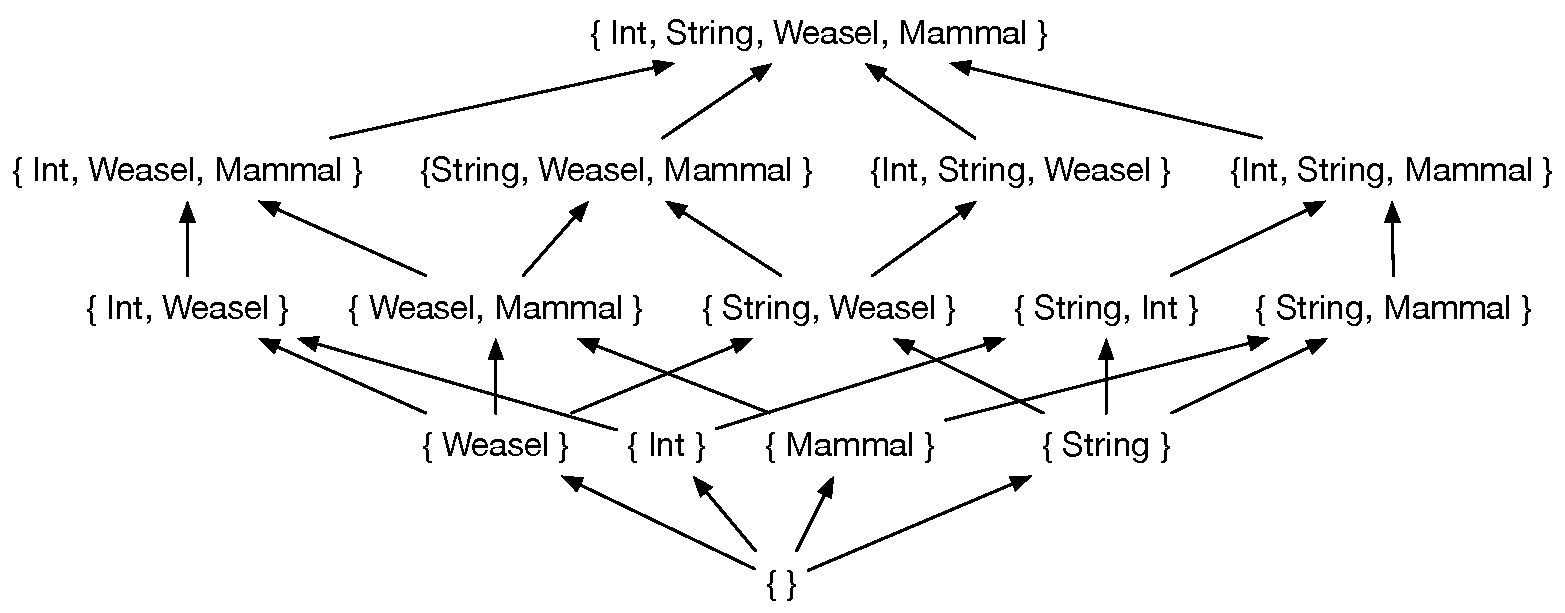
\includegraphics[scale=0.7]{img/Collecting-lattice.pdf}}
\caption{Subsets of types form a semi-lattice ordered by set
  inclusion.  In the example, Weasel is a subclass of Mammal.}
\label{fig-set-lattice}
\end{figure}

\subsection{An Abstract Semantics}

The collecting semantics is a little unwieldy, and it is also clumsy
to find a fixed point solution on sets of types, and then take the least
common ancestor of each set, and finally discover a type error.  We
can address both  problems by taking the least common ancestor
on-the-fly, using it as a representation for the set of types a
variable could take. 

There is no natural representation for the empty set of possible
types, but we can augment the type hierarchy with a special element
$\bot$ (pronounced ``bottom'') to represent ``no value yet''.  We can
also add an element $\top$ (pronounced ``top'') representing a type
error.  If we place these at the bottom and top of the hierarchy as
shown in Figure~\ref{fig-type-lattice}, the types form a lattice ordered
by the ``subtype of'' property. 

\begin{figure}
\centerline{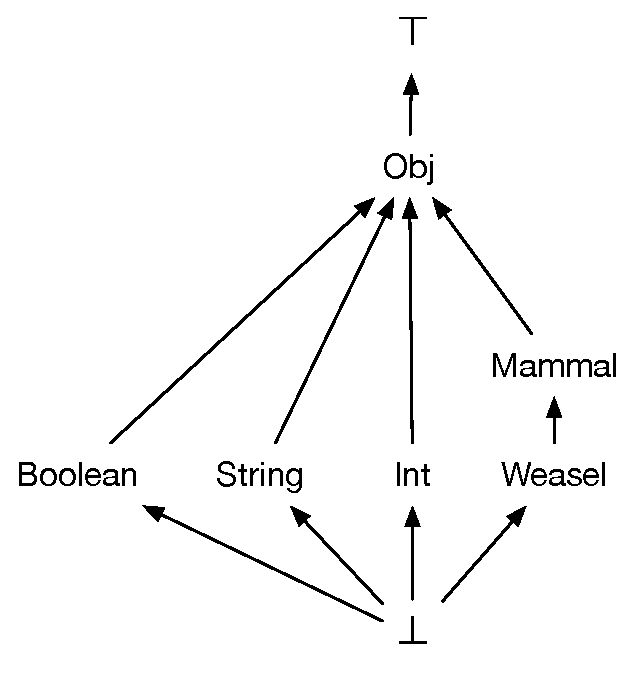
\includegraphics[scale=0.7]{img/Type-lattice.pdf}}
\caption{Types ordered by the ``subclass of'' relation, 
  augmented with an element $\bot$ for ``no information yet'' and
   $\top$ for ``type error'', form a lattice.  Compare to
   Figure~\ref{fig-set-lattice}. 
   Weasel is a subclass of Mammal.}
\label{fig-type-lattice}
\end{figure}


Like the lattice of sets ordered by ``subset of'', the lattice of
types ordered by ``subtype of'' has a property that is useful in
reasoning about correctness and termination of our type
inference.   Suppose we have an expression \( z.o(a_1, a_2, \ldots )\)
that gives us a type $T$ in environment $E$.  Now suppose we evaluate
the same expression in another environment $E'$ which is identical
except that some of the arguments $a'_i$ are supertypes of
corresponding $a_i$ in $E$.  It is not too hard to see that $T' \ge
T$, i.e., when the arguments to a method (including the receiving
object) go ``up'' in the lattice, the resulting type either stays the
same or goes up;  it cannot go down or ``across''.   (We added the
$\top$ element at the very top so that type errors would not be an
exception to this rule.)   
 We say that the
type inference rule is \emph{monotone}.   Being monotone, it ensures
that the computation of inferred static types converges (reaches a
fixed point) on the types we would have obtained using the sets of
types directly.  In fact it does so very rapidly, because the class
hierarchy in an object-oriented program is almost always quite
shallow.

\paragraph{We didn't want duck typing, anyway.}
It might seem at first that rejecting method \verb|not_duck_typing| is
a flaw in our type inference, or at least a disadvantage.  However,
using the least common ancestor rather than the set of possible types
has another advantage in addition to making type inference and type
checking easier:  It allows us to use a common implementation strategy
for dynamic method dispatch.  All the subclasses of a class with a
method \emph{foo} are no only guaranteed to have a compatible method
\emph{foo}  (either inherited or overridden), but in addition we will
implement those classes with a pointer to the code for \emph{foo} in
the same position in the class description.  The table of pointers to
methods in the class is sometimes called the \emph{vtable}, because in
C++ the methods in that table are called ``virtual functions'' or
``virtual methods.''  

\subsection{Putting it Together: Implementing Type Checking}

The abstract semantics above is the one you should implement.  You
will need an actual representation of the subtype hierarchy for all
the subtypes of \emph{Obj}.  The $\top$ and $\bot$ elements can be
implicit (which simplifies matters since the rest of the hierarchy is
a simple tree that can be represented by a table).  

You will want to create a table that maps from variables visible in a
method to the types of those variables.  Initially the arguments to
the method have their declared types, and all other variables have
type $\bot$.   

In pseudocode, the logic of the main type inference loop for a single 
method in Quack is roughly this, if 
\begin{verbatim}
  changed = true;
  while changed {
       changed = false;
       for each statement, in lexical order {
           type check the statement
       }
  }
\end{verbatim}

Of course I've hidden some complexity in the ``type check the
statement'' step.  Really it's not so complex, but each kind of Quack
statement and expression can require its own code.  We handle the type
of an expression exactly as we would do for the collecting semantics,
except that now we don't have to deal with sets of possible types, but
just with the current estimate of a type.  

For assignment statements, we don't just replace current type estimate
for a variable.  Rather, if we have previously estimated the type of a
variable to be T, and we now we are assigning type Q to that variable,
the new type is the \emph{least common supertype} of Q and T (i.e.,
their nearest ancestor in the tree).  Often, but not always, that will
be either Q or T.  Note that our estimate may ``move up'' the tree but
never down or across; and since the tree is finite,   this is our
guarantee that type inference will 
terminate.   If this results in a new type estimate for the variable,
we set the `changed' flag that controls the outer loop in the
pseudocode above. 

What if the assignment statement has a declared type, like 
\begin{verbatim}
x: Int = a + b;
\end{verbatim}

After
inferring a type for $a+b$, , we check that the inferred type is a subtype
(possibly equal).  If not, we report a type error.   Then we set the
estimated type to the declared type (even if it is a proper supertype
of the inferred type).  

\paragraph{Other statements.}
Besides assignments, Quack has while loops, if statements, return
statements, raw expressions, and typecase statements. 

\begin{itemize}
\item For while loops, we check that the condition evaluates to
  Boolean, and then we type check each statement in the body of the
  loop in the normal way. 
\item For if statements, we check that the condition evaluates to
  Boolean, and then we type check each statement in the true branch
  and the false branch. 
\item For return statements, we check that the expression evaluates to
  a some subtype of the method return type.   (In some cases this will
  be ``Nothing''.) 
\item For an expression that appears by itself, we calculate the type
  of the expression (because we might find a type error in the
  evaluation) and then discard it. 
\item Typecase is the most complex of the cases, and is considered
  brelow. 
\end{itemize}

\paragraph{Typecase}

A typecase statement is used to choose different code depending on the
dynamic type of an object, which may be a proper subtype of the static type of
the variable that holds it.   Consider: 
\begin{verbatim}
  def  EQUAL(other: Obj) : Boolean {
       typecase other {
         pt: Pt {  return this.x == pt.x and this.y == pt.y; }
       }
       return false;
  }
\end{verbatim}

We evaluate the typecase expression (\emph{other} in this example) and
discard the result; we only care that it it can be evaluated without a
type error.  Then, for each case (of which this example has only one),
we introduce a variable (like \emph{pt}) with the declared type
(\emph{Pt} in this case), and type check the statements within that
branch of the typecase in the augmented environment.  (Note that the
scope of the introduced variable is only for that branch of the
typecase.) 
           


\end{document}

